
En este capítulo se definirán los conceptos  o fundamentos de instrumentación estructural, sensores inteligentes y adquisición de datos, necesarios para llevar a cabo esta investigación.

\section{Estructuras civiles}

\subsection{Características generales}

Una estructura se refiere a un sistema de partes o elementos que se interconectan para cumplir una función es específico. En el caso de la ingeniería civil, suelen ser miembros que se utilizan para soportar una carga. Algunos ejemplos importantes son los edificios, los puentes y las torres; y en otras ramas de la ingeniería, son importantes las corazas de barcos y aviones, los sistemas mecánicos y las estructuras que soportan las líneas de transmisión eléctrica \citep{hibbeler1997structural}.

\subsection{Tipos de estructuras}

Según \citet{hibbeler1997structural}, cada sistema está formado por uno o varios de los cuatro tipos básicos de estructuras: 

\begin{itemize}
    \item Celosías.
    \item Cables y arcos.
    \item Armazones.
    \item Estructuras de superficie.
\end{itemize}

En general, estos elementos suelen soportar cargas, pueden ser estacionarios y también estar restringidos. Sus diferencias suelen basarse en la cantidad de fuerzas a las que están sujetos estos elementos en un instante dado.

La combinación de estos elementos y los materiales que los componen es lo que se denomina un sistema estructural. Estos sistemas, aunque sean pasados por alto, son utilizados diariamente por industrias y personas, siendo elementos claves en el desarrollo y progreso de la civilización actual.

\subsection{Comportamiento de las estructuras civiles}

La gran mayoría de los sistemas cuentan con una respuesta dinámica y estática. Ambas respuestas permiten conocer el comportaiento completo del sistema en estudio ante distintas entradas o en diferentes situaciones. Al estudiar el comportamiento estructural se encuentra una extensa literatura tanto para el estudio dinámico como para el régimen estático, recopilándose lo siguiente:

\begin{itemize}
    \item{Respuesta estática}: En la ingeniería civil toda estructura se diseña para que se encuentre en reposo cuando actúan sobre esta fuerzas externas, es decir, la estructura en conjunto debe cumplir con las condiciones de equilibrio, siendo la fuerza y el momento resultanto sobre esta igual a cero en todo momento. Para describir estas condiciones de equilibrio se cuentan con herramientas matemáticas que proporcionan las condiciones necesarias para su cumplimiento. Estas ecuaciones permiten la resolución estática de la estructura, la cual permite determinar el valor de todas las incógnitas estáticas de interés \citep{basset2014analisis}.
    
    \indent Cuando las fuerzas que actúan sobre la estructura pueden calcularse a partir de las ecuaciones de equilibrio, se tiene una estructura en equilibrio y se denonima estructura estáticamente determinada. En caso de tenerse más fuerzas desconocidas que ecuaciones de equilibrio se habla de una estructura estáticamente indeterminada.

        \begin{itemize}
            \item Rigidez: Uno de los parámetros más importantes dentro de la respuesta estática es la rigidez. Esta se define como la propiedad que tiene un elemento estructural de soportar la deformación o deflección al estar bajo la acción de una fuerza o carga. Una medida de la rigidez viene dada por el Módulo de Young; esta es una constante del material y es independiente de la cantidad de material.
        \end{itemize}

    \item{Respuesta dinámica}: La dinámica estructural se encarga de estudiar el efecto que tienen cargas dinámicas sobre el sistema. La respuesta ante estos eventos, como pueden ser sismos, vientos, equipos mecánicos, paso de vehículos o personas, se denomina respuesta dinámica \citep{hurtado2000}. Además, la respuesta dinámica permite caracterizar algunos parámetros de gran interés para estudiar su comportamiento conocidos como parámetros modales. Estos parámetros surgen al estudiar las ecuaciones diferenciales que describen el movimiento de la estructura, partiendo de un modelo idealizado simple de masa concentrada como el de la Figura \ref{fig:masa_estructural}.
    
    \begin{figure}[H]
        \centering
        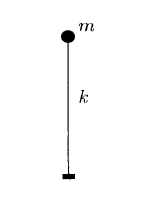
\includegraphics[width = 0.25\textwidth]{imagenes/cap1_marcoteo/modelo_masa_simple.png}
        \caption{Modelo de masa concentrada de 1 grado de libertad \citet{hurtado2000}.}
        \label{fig:masa_estructural}
    \end{figure}

    La dinámica de este modelo puede describirse utilizando la ecuación diferencial de movimiento:

    \begin{equation} \label{eq:vib_lib}
        m\ddot{u} + f_R(t) = p(t)
    \end{equation}

    La ecuación \ref{eq:vib_lib} se conoce como ecuación de vibración libre sin amortiguamiento. Donde $p(t)$ representa las cargas dinámicas y $f_R(t)$ la fuerza de restitución propia de un material elástico.  Esta ecuación es una ecuación diferencial de coeficientes constantes, que consta de una solución homogénea más una solución particular. La solución homogénea será la respuesta de la estructura a la vibración libre, es decir, si la masa de la Figura \ref{fig:masa_estructural} se deja oscilar libremente.

    Se sabe que una ecuación de este tipo tendrá una solución como:

    \begin{equation} \label{eq:sol_equ_dif}
        u = A.sin\omega t + B.cos\omega t
    \end{equation}

    La ecuación \ref{eq:sol_equ_dif} contiene información relevante para la caracterización dinámica de la estructura. Esta caracterización parte del estudio de los parámetros modales de la misma.

    Entre estos parámetros modales se encuentran: 
        \begin{itemize}
            \item Frecuencia natural: Toda estructura física tiene asociada una frecuencia de vibración natural. Las máquinas, los puentes, los edificios; todas estas estructuras vibran u oscilan al ser perturbadas o removidas de su estado de reposo inicial. Es una propiedad es intrínseca del sistema y depende de su masa, rigidez y amortiguamiento. Todas tienen al menos una frecuencia natural y es posible que tengan múltiples frecuencias de resonancia \citep{irvine2000introduction}. 
            
                Se suele calcular la frecuencia natural de resonancia de un sistema libre usando:

                \begin{equation}
                    f =  \frac{1}{\sqrt{\frac{k}{m}}}
                \end{equation}

            \item Amortiguamiento: Toda estructura comienza a oscilar una vez es removida de su estado de reposo o equilibrio, sin embargo, ese movimiento no es perpetuo. El amortiguamiento se define como la capacidad de disipación de energía que posee la estructura bajo excitaciones externas. Las soluciones a la ecuación \ref{eq:vib_lib}, al añadir el amortiguamiento de tipo viscoso, arrojan 3 posibles casos:
                \begin{enumerate}
                    \item Sistema críticamente amortiguado: El sistema no vibra.
                    \item Subamortiguado o amortiguado subcrítico: Caso más común por la naturaleza de los materiales utilizados en las estructuras. La respuesta del sistema decae con el tiempo de forma exponencial, como se puede ver en la Figura \ref{fig:resp_subamorti}. 
                    
                    \begin{figure}[H]
                        \centering
                        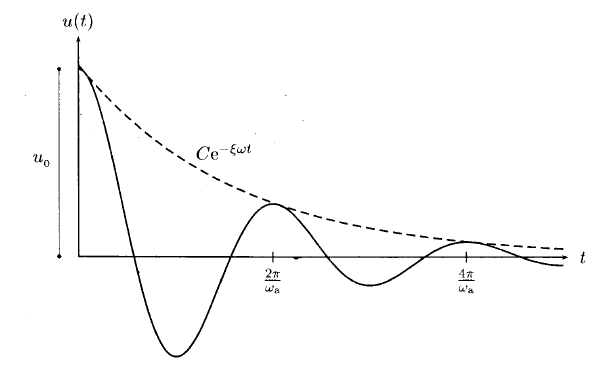
\includegraphics[width = 0.7\textwidth]{imagenes/cap1_marcoteo/respuesta_sist_subamorti.png}
                        \caption{Respuesta ante vibración libre en sistema Subamortiguado \citep{hurtado2000}.}
                        \label{fig:resp_subamorti}
                    \end{figure}

                    \item Sobreamortiguado: Nunca se encuentra esta respuesta en sistemas estructurales por los materiales utilizados.
                \end{enumerate}
            
        \end{itemize}        
\end{itemize}

\subsection{Respuesta en frecuencia}

    Incluir?

\subsection{Daño en estructuras}

El daño a una estructura civil o mecánica puede definirse como todo cambio en las propiedades materiales o geométricas del material que llegan a afectar de forma adversa la confiabilidad y el desempeño actual o futuro del sistema. Por tanto, el daño es una comparación entre el sistema en cuestión en 2 instantes de tiempo distintos \citep{farrar2007introduction}. Estos efectos adversos pueden ser, en el caso estructural, desplazamientos, estrés indeseado en un elemento o vibraciones estructurales indeseadas \citep{chen2018}.

Toda estructura civil, como puentes y edificios, acumulan daño de forma continua a medida que están en servicio y transcurre su vida útil. Este daño puede manifestarse como fracturas, fatiga, socavaciones o desprendimiento del concreto. El daño que no sea detectado puede conducir a una falla estrcutural que a su vez ocasione pérdidas humanas. Por tanto, es imperativo y necesario detectar el daño en una estrcutrura tan pronto como sea posible, \citep{chen2018}.

Entre algunos de los factores que influyen del deterioro de una estructura se encuentran:
    
        \begin{itemize}
            \item Proceso de degradación natural de los materiales.
            \item Corrosión del acero de refuerzo.
            \item Evento sísmico, incendios o condiciones de guerra.
            \item Carga por encima del límite de diseño.
        \end{itemize}
    
Las escalas de tiempo y de extensión del daño son diversas. Por ejemplo, el deterioro por el paso del tiempo bajo ciertas condiciones climáticas es muy lento comparado al daño causado por un evento catastrófico.

\subsection{Principios de la Sismoresistencia}

Una edificación sismorresistente es aquella que está diseñada y construida para soportar las fuerzas causadas por eventos sísmicos. Sin embargo, incluso las edificaciones diseñadas y construidas según las normas sismorresistentes pueden sufrir daños en caso de un terremoto muy fuerte, sin embargo, las normas establecen los requisitos mínimos para proteger la vida de
las personas que ocupan la edificación

Algunas de las características de una estructura sismoresistente son:

        \begin{itemize}
            \item Forma regular.
            \item Bajo peso.
            \item Mayor rigidez.
            \item Buena estabilidad.
            \item Suelo firme y buena cimentación.
            \item Materiales competentes.
            \item Capacidad de disipación de energía.
            \item Fijación de acabados e instalaciones.
        \end{itemize}

En Venezuela las estructuras deben cumplir con la Norma Venezolana COVENIN 1756:2001 (Edificaciones Sismorresistentes).

Se ha observado que al estudiar el comportamiento de las estructuras luego de un evento sísmico, es evidente que cuando se toman en cuenta las normas de diseño sismorresistente dispuestas en la ley y la construcción es debidamente supervisada, los daños estructurales resultan ser considerablemente menores que en las edificaciones en las cuales no se cumplen los requerimientos mínimos indispensables estipulados en la norma, \citep{blanco2012criterios}.

\subsubsection{Importancia de la instrumentación} La instrumentación estructural permite medir y monitorear las acciones y respuestas estructurales ante distintos eventos. Esto proporciona datos en tiempo real sobre el comportamiento dinámico y estático de la estructura, como deformaciones, aceleraciones y desplazamientos, que son fundamentales para evaluar y verificar si la estructura cumple con los criterios de diseño sismoresistente establecidos en la norma.

La instrumentación estructural ayuda a validar los modelos y suposiciones utilizados en el diseño estructural inicial. Al comparar los datos recopilados por la instrumentación durante un evento sísimco con las predicciones del modelo, es posible verificar si la estructura se comporta de acuerdo con las expectativas y si cumple con los criterios de seguridad establecidos en la normas.

Además, el monitoreo continuo de la estructura permite conocer el estado actual de la misma, tema que representa la idea principal del Monitoreo de Salud Estructural, permitiendo a los ingenieros evaluar si se sigue cumpliendo con la norma para luego tomar decisiones y actuar en pro de la seguridad de la edificación.


\section{Salud estructural}

\subsection{Definición}


El proceso de implementar una estrategia de identificación de daño para estructuras civiles, mecánicas o aeroespaciales se conoce como Monitoreo de Salud Estructural (SHM por sus siglas en inglés). Esta estrategia requiere medir las condiciones y el ambiente en el que opera la estructura, además de la respuesta de la misma durante un período de tiempo tomando muestras periódicamente espaciadas, \citep{farrar2007introduction}.


La estrategia del SHM requiere de equipos multidisciplinarios de ingeniería, ya que necesita de una red de sensores que midan las variables de interés, el procesamiento y análisis de los datos obtenidos y posteriormente una prognosis del daño para una eventual toma de decisiones. El objetivo del SHM es proveer, en toda la vida útil de la estructura, un diagnóstico del estado de sus materiales constitutivos, de los diferentes elementos que la componen y de la estructura en sí como el conjunto de todas estas partes. Esto para garantizar que la misma se comporte dentro de los parámetros iniciales de diseño, aunque estos cambien por la acción natural del tiempo, el ambiente y accidentes, \citep{balageas2010structural}.

El resultado de este proceso es información actualizada sobre el estado de la estructura y sobre su capacidad actual para seguir desempeñado la función para la cual fue diseñada.

Según \citet{enckell2006structural}, el SHM se ha convertido en una herramienta muy conocida y utilizada en ingeniería estructural en los últimos años en diferentes países.

\subsection{Reseña histórica}

Las técnicas de detección de daño basadas en vibración tienen sus primeras aplicaciones desde hace cientos de años. En la antigüedad, los constructores golpeaban las estructuras para encontrar espacios vacíos o grietas en elementos de arcilla. La utilidad de estas inspecciones tan simples indicaban que la sofisticación de estos métodos podía proveer información muy valiosa sobre el elemento de interés, sin embargo, esto requiere de instrumentos y herramientas matemáticas que se han desarrollado con el pasar de los años. El auge en el uso de SHM en años recientes es consecuencia de la evolución y miniaturización del hardware computacional actual.


El uso más exitoso del SHM ha sido el monitoreo de la condición de máquinas rotativas, las cuales actualmente han adoptado un enfoque de indetificación de daño sin basarse en un modelo de forma casi exclusiva, \citep{farrar2007introduction}.

En los años 70 la industria petrolera consideró el uso de técnicas basadas en vibración para identificar daños en plataformas costa-afuera, este enfoque se diferenció de las máquinas rotativas al estudiar un sistema en donde la ubicación del daño es desconocida y difícil de instrumentar.

En esa misma época, la comunidad aeroespacial y la \textit{National Eeronautics Space Agency} (NASA), comenzaron a estudiar esta técnica de identificación de daño en los comienzos de la era de lanzamientos espaciales. Este trabajo continúa hoy en día y el \textit{Shuttle Modal Inspection System} (SMIS) se desarrolló para identificar fatiga en distintos componentes de cohetes espaciales reusables, los cuales representan el futuro de esta industria.


Usualmente, los enfoques de estas industrias se basan en comparar modelos analíticos de estructuras sin daño con las mediciones de estructuras con daño, observando principalmente las propiedades modales de las mismas. Se ha observado que cambios en la rigidez en ambos modelos han permitido localizar y cuantificar el daño, \citep{farrar2007introduction}.

Inicialmente, las técnicas no destructivas fueron introducidas en la ingeniería civil a mediados de los años 40, \citep{mohamed2014}. La necesidad principal surgió en determinar propiedades del concreto fresco \textit{in-situ}. Estas técnicas, que buscaban evaluar la homogeneidad y la resistencia del concreto eran en su mayoría pruebas con martillo y pruebas de \textit{pull-out}. A medida que las estructuras envejecieron, los ingenieros necesitaban idear maneras de medir o estimar las propiedades mecánicas de los elementos que consituyen las estructuras, además de detectar daños que no eran fáciles de observar por la envergadura de las estructuras civiles que se han desarrollado en los últimos 150 años. Es ahí, en los años 70, donde surgen nuevas estrategias no destructivas tales como:

    \begin{itemize}
        \item Emisión acústica.
        \item Métodos de ultrasonido y radar.
        \item Termografía.
        \item Métodos basados en vibración
    \end{itemize}

La comunidad de ingeniería civil ha estudiado la identificación de daño basada en vibración en puentes y edificios desde comienzos de los años 80. Las propiedades modales han sido estudiadas por diferentes autores y son las principales características que se analizan al identificar daño. El auge del SHM es tal, que algunos países asiáticos han implementado regulaciones en donde las compañías constructoras deben verificar la salud estructural de los puentes periódicamente. Estas regulaciones han provocado que la investigación e inversión en esta área siga aumentando de forma considerable, \citep{chen2018}. 

\subsection{Línea de trabajo del Monitoreo de Salud Estructural}

Los sistemas de SHM consisten de varios elementos que permiten a los ingenieros tener información sobre el estado de una estructura, entre esos elementos se encuentran:

\begin{itemize}
    \item Sensores.
    \item Sistemas de adquisición de datos.
    \item Sistema de transmisión de datos.
    \item Sistema de procesamiento de datos.
    \item Sistema de manejo y almacenamiento de datos.
    \item Equipo de análisis y toma de decisiones.
\end{itemize}

\begin{figure}[H]
    \centering
    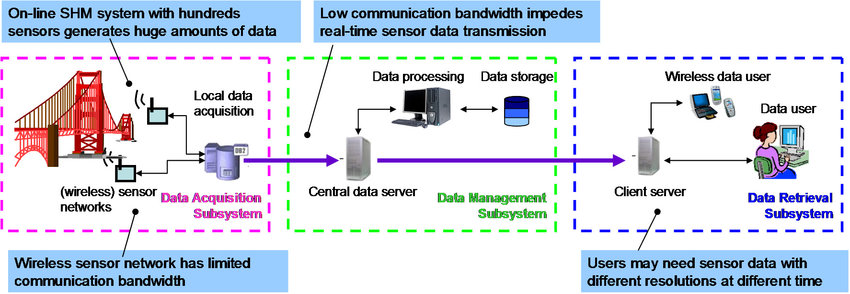
\includegraphics[width = 0.9\textwidth]{imagenes/cap1_marcoteo/Schematics-of-an-on-line-structural-health-monitoring-system-and-technical-challenges.png}
    \caption{Esquema de un sistema de SHM \citep{lijianfoto2015}.}
    \label{fig:esquema_gral_SHM}
\end{figure}


Autores como \citet{rytter1993vibration} y \citet{farrar2007introduction} han esquematizado la estrategia del SHM categorizando el daño en una estructura por niveles de la siguiente forma:

\begin{enumerate}
    \item Nivel I (detección del daño) ¿Presenta daño el sistema? Es una indicación cualitativa de que puede haber daño presente en la estructura.
    \item Nivel II (localización o ubicación del daño) ¿Dónde está presente el daño? Indica la posible localización del mismo. 
    \item Nivel III (clasificación del daño) ¿Qué tipo de daño está presente? Da información sobre el tipo de daño.
    \item Nivel IV (alcance/grado/extensión del daño) ¿Cuál es el alcance del daño? ¿Qué tan grave es? Da un estimado del alcance.
    \item Nivel V (prognosis del daño) ¿Cuánta vida útil le queda a la estructura? Da un estimado de la seguridad de la estructura.
\end{enumerate}

En la mayoría de los casos, para alcanzar el nivel final es necesario obtener información sobre los niveles previos. Esto indica que a medida que se sube de nivel se tiene un mayor conocimiento sobre el estado de la estructura.

De acuerdo a \citet{chen2018}, los primeros dos niveles, detección y localización, generalmente pueden alcanzarse usando métodos de detección basados en vibración para obtener mediciones sobre la respuesta dinámica de la estructura.

Por su parte, \citet{chen2018} describe el proceso de SHM en general como:

\begin{enumerate}
    \item Observación.
    \item Evaluación.
    \item Calificación.
    \item Gestión.
\end{enumerate}

La estrategia de Monitoreo de Salud Estructural podría resumirse en el siguiente diagrama:

\begin{figure}[H]
    \centering
    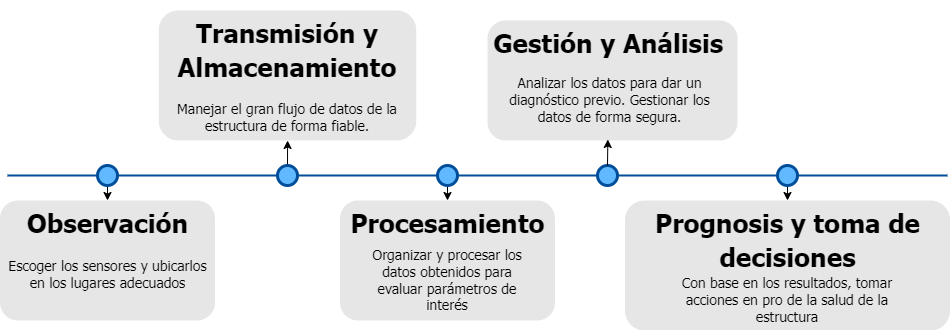
\includegraphics[width = \textwidth]{imagenes/cap1_marcoteo/Diagrama SHM timeline.png}
    \caption{Diagrama general del proceso de SHM.}
    \label{fig:diag_SHM}
\end{figure}

\subsection{Criterios de evaluación}

Como se definió anteriormente, el daño estructural puede tener distintas causas y formas. Lo que se sabe con certeza es que una estructura, una vez entra en funcionamiento, análogo a los seres humanos al nacer, estará sujeta a envejecimiento natural y a condiciones adversas. Ahora bien, en el caso del SHM, surge la siguiente pregunta ¿Qué se debe medir para poder detectar este daño?. 

Numerosos autores concluyen que uno de los indicativos de daño de una estructura viene dado por los parámetros modales definidos anteriormente, frecuencia y amortiguamiento. Esta relación entre los parámetros modales y el daño viene dada por la premisa de que todo daño presente en la estructura se reflejará en un cambio en las propiedades dinámicas de la misma. \citet{worden2009modal}, comprobó la relación entre el cambio progresivo en todas las frecuencias naturales de 15 vigas estudiadas a las cuales se les introdujo un daño relacionado con un cambio del Módulo de Young, el cual, como fue mencionado anteriormente, provee un indicativo de la rigidez de un elemento.

Anterioremente en la ecuación \ref{eq:vib_lib} se definió un sistema con un grado de libertad (DOF por sus siglas en ingles), sin embargo, en la realidad las estructuras tienen múltiples grados de libertad, por lo que es conveniente modelarlas de estar forma para obtener resultados más precisos. En el caso de los sistemas \textit{n-dregrees of freedom} (DOF por sus siglas en ingles), la ecuacion de movimiento que describe la dinámica del sistema en vibración libre vendrá dada por:

\begin{equation} \label{eq:ecu_movimiento}
    M\ddot{u} + C\dot{u} + Ku = 0
\end{equation}

Donde M, C y K representan las matrices de masa, amortiguamiento y rigidez de la estructura, respectivamente.

Si se asume un sistema sin amortiguamiento, a fines de estudiar el efecto que tiene sobre la rigidez un cambio en los parámetros modales,  de la ecuación \ref{eq:ecu_movimiento} se obtiene: 

\begin{equation} \label{eq:ecu_movimiento_sindamp}
    M\ddot{u} + Ku = 0
\end{equation}

Si se asume una solución oscilatoria pura, por ser un sistema sin amortiguamiento:

\begin{equation} \label{eq:sol_ecu_motion}
    u = ve^{jwt}
\end{equation}

Al derivar, sustituir y despejar en la ecuación \ref{eq:ecu_movimiento_sindamp} se obtiene:

\begin{equation} \label{eq:eig_problem}
    (K - \lambda M)\phi = 0
\end{equation}

Esta ecuación \ref{eq:eig_problem} representa claramente un problema de autovalores, donde $\lambda$ representa los autovalores asociados a las frecuencias naturales del sistema y $\phi$ representa el autovector de desplazamiento.

Si se introduce un pequeño cambio $\Delta K$ con perturbaciones similares en los otros parámetros:

\begin{equation}
    [(K - \Delta K) - (\lambda - \Delta\lambda)(M - \Delta M)](\phi - \Delta\phi) = 0
\end{equation}

El daño estructural suele venir asociado a un cambio en la rigidez, mas no a cambios en la masa de la estructura, por lo que se asume $\Delta M = 0$, \citep{hearn1991modal}. A su vez, se tiene que $(K - \lambda M)\phi = 0$. \citet{mohamed2014}, \citet{shi1998structural} y \citet{hearn1991modal} desarrollan estas ecuaciones obteniendo la siguiente relación:

\begin{equation} \label{eq:relacion_final}
    \Delta\lambda = \phi^T \Delta K \phi
\end{equation}

De la ecuación \ref{eq:relacion_final} se observa que cambios en los autovalores $\lambda$ que representan las frecuencias naturales, y en los autovectores $\phi$ (formas modales) están directamente relacionados con cambios en la matriz de rigidez (K) del sistema. De aquí surge el interés en monitorear los parámetros modales como indicadores de daño estructural. Es importante recalcar que estos cambios son indicativos de daño global, mas no de la localización del mismo, para lo que se necesitan otras técnicas, \citep{mohamed2014}.

\subsection{Variables de interés}

Tomando en cuenta la relación entre los parámetros modales y el daño presente en una estructura, es preciso definir las variables de interés para el monitoreo de la salud estructural de una estructura. Si bien existen distintas varibales que permiten obtener información valiosa sobre la estructura en estudio, algunas de estas no proporcionan información global del daño, como es el caso de las formas modales y la deflección local \citep{rytter1993vibration}. Sin embargo, estas mediciones proveen indicativos de la ubicación del daño, por lo que pueden constituir parte del sistema de monitoreo en una etapa más avanzada, es decir, una vez el daño fue detectado. A continuación se presentan las más relevantes para el daño global:

    \begin{itemize}
        \item Frecuencias naturales y amortiguamiento: Los parametros modales de la estructura están ligados de forma directa al estado de la misma. El deterioro en una edificiación induce cambios en la rigidez estructural, como se observa claramente en la ecuación \ref{eq:relacion_final}. El daño puede tener efectos distintos en cada modo o cada frecuencia de vibración, por lo que es importante no ubicar los sensores sobre los nodos modales, ya que experimentos han demostrado la ineficacia en las mediciones. Usualmente, el daño se refleja como una disminución en las frecuencias naturales afectadas, aunque se han observado casos de aumento en las frecuencias de vibración en estructuras de concreto pretensado, \citep{rytter1993vibration}.
        
        A su vez, el amortiguamiento varía al introducir daño en la estructura, puesto que su capacidad de disipar energía se ve afectada. Usualmente, los investigadores observan un aumento en el amortiguamiento a medida que el daño aumenta, como se ha demostrado experimentalmente por autores como \citet{hearn1991modal} y \citet{rytter1993vibration}.

        \item Temperatura y humedad: En los sistemas de monitoreo, la detección del daño estructural puede tomar períodos de tiempo considerables, durante los cuales las caracterpisticas sujetas a temperatura y humedad, sufren cambios que afectan la respuesta estructural.
                
        Es evidente que las condiciones climáticas contribuyen con el deterioro de las edificaciones. A pesar de esta conclusión, relacionar las condiciones climáticas con el daño introducido usando mediciones ambientales es difícil. La medición de estas variables suele tomarse en cuenta para poder cuantificar el cambio que producen estas condiciones en los demás indicadores de daño. \citet{rytter1993vibration} observó que la humedad y temperatura afectaban las mediciones de amortiguamiento. Por su parte, \citet{mohamed2014}, observó que las frecuencias naturales de barras y vigas disminuían a medida que aumentaba la temperatura. A su vez, \citet{sohn2007effects} determinó que cuando hay humedad, los puentes de hormigón absorben una cantidad considerable de humedad, lo que aumenta sus masas y altera sus frecuencias naturales.
        
        \item Inclinación y desplazamiento: n practical applications of structural monitoring, the most common is the measurement of linear displacements, which reflect in a very good and direct way the behavior of the structural element / structure or a part of the structure.
        
        Inclinometers are used to measure inclination (tilt) of structural components due to distress in the system. For example, they are often utilised to assess fixity of bridge girders at supports and to monitor longterm movements of bridge piers, abutments and girders.

        Deflection is a very important index for bridge structures, because it not only affects driving comfort, but also reflects the overall response of the bridge. Various factors could contribute to deflection increase during bridge service life, such as concrete creep, steel corrosion, prestress loss, and crack growth. The increase of structural deflection, however, will in turn accelerate the damage accumulation process. Therefore, monitoring bridge deflection is of great significance in the field of structural health monitoring (SHM) to provide early warnings of possible structural changes, damage, or deterioration.

        In several industries during the last few decades, inclinometer sensors have been employed extensively. In fact, in the civil engineering sector, inclinometers were initially used for geotechnical purposes [80]. Improvements in sensor accuracy over time have made it possible to use inclinometers in other areas of civil engineering, such as monitoring the structural health of bridges [79].
        


    \end{itemize}
    

\subsection{Consideraciones y desafíos}

\section{Sensores}

\subsection{Definición y tipos de sensores}

\subsection{Sensores de interés para el Monitoreo de Salud Estructural}

    \begin{itemize}
        \item Acelerómetros e Inclinómetros:
        \item Desplazamiento:
        \item Temperatura:
        \item Humedad:
    \end{itemize}

\subsection{Sensores inteligentes}

\section{Microcontroladores}